% Created 2023-10-04 Mi 16:19
% Intended LaTeX compiler: pdflatex
\documentclass[11pt]{article}
\usepackage[utf8]{inputenc}
\usepackage[T1]{fontenc}
\usepackage{graphicx}
\usepackage{longtable}
\usepackage{wrapfig}
\usepackage{rotating}
\usepackage[normalem]{ulem}
\usepackage{amsmath}
\usepackage{amssymb}
\usepackage{capt-of}
\usepackage{hyperref}
\usepackage{parskip}
\setcounter{secnumdepth}{2}
\setcounter{tocdepth}{2}
\usepackage{titlesec}
\titleformat{\section}{\newpage \normalfont\large\bfseries}{Chapter \thesection}{1em}{}
\providecommand{\xmapsto}[1]{\overset{#1}{\longmapsto}}
\providecommand{\bra}[1]{\langle#1|}
\providecommand{\ket}[1]{|#1\rangle}
\providecommand{\braket}[2]{\langle#1|#2\rangle}
\providecommand{\ketbra}[2]{|#1\rangle\langle#2|}
\providecommand{\proj}[1]{|#1\rangle\langle#1|}
\providecommand{\av}[1]{\langle#1\rangle}
\providecommand{\tr}{\operatorname{tr}}
\providecommand{\id}{\mathbf{1}}
\providecommand{\diag}[2]{\begin{bmatrix}#1&0\\0&#2\end{bmatrix}}
\providecommand{\smalldiag}[2]{\left(\begin{smallmatrix}#1&0\\0&#2\end{smallmatrix}\right)}
\providecommand{\mqty}[1]{\begin{matrix}#1\end{matrix}}
\providecommand{\bmqty}[1]{\begin{bmatrix}#1\end{bmatrix}}
\newcommand{\myvec}[1]{\ensuremath{\begin{bmatrix}#1\end{bmatrix}}}
\renewcommand{\leq}{\leqslant}
\renewcommand{\geq}{\geqslant}
\usepackage{todonotes}
\usepackage{amsthm}
\usepackage{amsmath}
\usepackage[left=3cm,right=2cm,top=3cm,bottom=2cm,includeheadfoot]{geometry}
\usepackage{txfonts} % TX Serif and Sans (Helvetica)
\usepackage{lmodern}
\usepackage{graphicx}
\usepackage{xcolor}
\usepackage{uni-titlepage}
\usepackage{glossaries}
\usepackage{url}
\makeglossaries
\theoremstyle{definition}
\newtheorem{exmp}{Example}[section]
\theoremstyle{definition}
\newtheorem{definition}{Definition}[section]
\newglossaryentry{zx}{name=ZX-Calculus,description={{A graphical calculus used in quantum computing}}}
\newglossaryentry{tdd}{name=Tensor Decision Diagrams,description={{A data structure used in quantum computing for optimization}}}
\newglossaryentry{dqc}{name=Dynamic Quantum Circuit,description={{A type of quantum circuit that contains non-unitary operations}}}
\newglossaryentry{qct}{name=Quantum Circuit,description={{A traditional quantum circuit}}}
\newglossaryentry{qce}{name=Quantum Circuit Equivalence Checker,description={{A tool for checking the equivalence of quantum circuits}}}
\newglossaryentry{pycl}{name=PyCall,description={{A Julia library for integrating with Python}}}
\newglossaryentry{mqtqc}{name=mqt-qcec,description={{An equivalence checker for quantum circuits}}}
\newglossaryentry{qiskit}{name=Qiskit,description={{A widely used quantum computing framework}}}
\newglossaryentry{qubit}{name=Qubit,description={{A fundamental unit of quantum information}}}
\newacronym{mqt}{}{Munich Quantum Toolkit}
\newacronym{jl}{Julia}{Julia programming language}
\newacronym{qcec}{QCEC}{Quantum Circuit Equivalence Checker}
\newacronym{qasm}{QASM}{OpenQASM file format}
\date{\today}
\title{Analysis of ZX-Calculus Tools for Efficient Verification of Static and Dynamic Quantum Circuits}
\hypersetup{
 pdfauthor={Liam Hurwitz},
 pdftitle={Analysis of ZX-Calculus Tools for Efficient Verification of Static and Dynamic Quantum Circuits},
 pdfkeywords={},
 pdfsubject={},
 pdfcreator={Emacs 29.1 (Org mode 9.6.6)}, 
 pdflang={English}}
\begin{document}

\pagenumbering{roman}
\begin{titlepage}
    \centering
    
\includegraphics[width=0.25\textwidth]{img/logo_uni_bremen}\par\vspace{1cm}
  %%  {\textsc{Universität Bremen} \par}
  %%  \vspace{1cm}
    {\Large \textsc{Bachelor Thesis}\par}
    \vspace{1.5cm}
    {\huge\bfseries Analysis of ZX-Calculus Tools for Efficient Verification of Static and Dynamic Quantum Circuits\par}
    \vspace{2cm}
    {\Large\itshape Liam Hurwitz\par}
    \vfill
    supervised by\par
  Prof. Dr.~Rolf \textsc{Drechsler}\par
  Dr.~Kamalika \textsc{Datta}\par
  Dr.~Abhoy \textsc{Kole}\par

    \vfill

% Bottom of the page
    {\large \today\par}
\end{titlepage}

\newpage
\tableofcontents \clearpage
\pagenumbering{arabic}
\newpage
\addtocounter{page}{0}

\section*{Abstract}
\label{sec:orgf972655}
TBW


\section{Introduction}
\label{sec:orgd11bd8c}
Quantum Computing is a rapidly advancing field that has the potential to
revolutionize the way we solve complex problems \cite{de_potential_2017}.
It theoretically offers several benefits over classical computers.
In the future a large quantum computer could break widely used encryption schemes,
which rely on functions that are easy to compute in one direction, yet
difficult to compute in the opposite direction or aid physicists to simulate
quantum objects without the overhead, that arises when using classical
computers \cite{feynman_simulating_1982}\cite{nielsen_quantum_2010}.


In 2019 researchers claimed to have demonstrated the quantum advantage
\cite{arute_quantum_2019},
showing that quantum computers have the potential to solve complex problems,
such as optimizing complex systems or simulating complex phenomena
much more efficiently than a classical computer could \cite{preskill_quantum_2018}.

Quantum Computers take advantage of quantum mechanical phenomena, such
as superposition and entanglement, to solve problems that are difficult or
impossible for classical computers \cite{hayashi_introduction_2015}
and have changed our understanding of computability.
Contrary to classical information theory computation is not
self-evident and abstract, but a physical process
\cite{sep-computation-physicalsystems_2021}.
Information is stored, transmitted and processed by physical methods \cite{deutsch_quantum_1985}.


Currently, we are in the NISQ era, short for \emph{Noisy Intermediate Scale Qubits}.
Current quantum devices contain up to a \(1000\) qubits, but are not advanced enough
for fault-tolerance \cite{preskill_quantum_2018}.
The long-term goal in quantum computation is to reach \emph{Fault Tolerant Quantum Computing},
were we will see more applications and benefits arise.
Due to the limited number of qubits available in the NISQ hardware
architecture, it is not possible to map any impactful quantum algorithm onto
these architectures or available quantum devices \cite{almudever_realizing_2020}.

With the introduction of non-unitary operations such as mid-circuit
measurement, active resets and classical controlled quantum operations,
a new class of circuits known as Dynamic
Quantum Circuits (DQC) has evolved \cite{corcoles_exploiting_2021}, bringing
us one step closer to overcome limitations of near-term quantum devices by
reducing the number of qubits.
Existing quantum circuits equivalence checking tools require an
evaluation to see if they are capable of efficiently verifying the equivalence of
Dynamic Quantum Circuits \cite{burgholzerHandlingNonunitariesQuantum2022}.
\subsection{Quantum Computers}
\label{sec:org4de1618}
A quantum computer is a computer which exploits quantum mechanical phenomena.
Using specialized hardware, which supports the preparation and manipulation
of quantum states, quantum computers utilize the concept of the
wave-particle duality, specifically quantum superposition and entanglement \cite{nielsen_quantum_2010}.
This quantum mechanical concept states that at a small scale physical matter
exhibits properties of both particles and waves \cite{messiah_quantum_1999}. Neither the classical concept
of ``particle'' or ``wave'' are able to describe the behaviour of quantum objects \cite{feynman_quantum_2007}.

Quantum devices continue to advance steadily, with notable enhancements in
both capability and accessibility.
A variety of quantum computing platform, such as IBM Q \cite{cross_ibmq_2018}, Microsoft Q\# \cite{hooyberghs_qsharp_2022} and Amazon Bracket \cite{gonzalez_cloud_2021}
are remotely accessible to researchers and the public, sometimes even for free.
These quantum computers are used in diverse applications, from simulating
quantum systems to solving complex optimization problems.

\subsubsection{Advantages over Conventional Computation}
\label{sec:orgd20e6ae}
Quantum computing has several advantages over conventional computing, including:
\begin{description}
\item[{Runtime of Algorithms}] Quantum algorithms can solve certain problems faster
than classical algorithms, even when the problem size is increased. This
means that quantum computers can solve problems more efficiently than
classical computers, which is important for applications where computational
power is limited \cite{montanaro_quantum_2016}.
\item[{Quantum Supremacy}] Quantum computers can solve problems that would
take to long to compute on classical computers. This means that quantum computers can
solve problems that are currently unsolvable with classical computers, due to the
large time complexity of these problems \cite{preskill_quantum_2012}. This has significant implications for
many research fields.
\item[{Quantum algorithms (Shor or Grover)}] Quantum computers can use algorithms
such as Shor's algorithm \cite{shor_poly_1997} and Grover's algorithm
\cite{grover_fast_1996} to solve problems that are very difficult or
impossible for classical computers to solve. These algorithms take advantage
of quantum mechanical phenomena, such as superposition and entanglement
\cite{jozsa_entanglement_1997}, to solve problems more efficiently than
classical algorithms \cite{nielsen_quantum_2010}.
\end{description}

In conclusion, quantum computing offers several benefits over classical
computing, including the ability to solve complex problems more efficiently
and the potential to solve problems that are beyond the capabilities of
classical computers. These advantages make quantum computing an essential
area of research with potential applications in a wide range of fields.

\subsubsection{Unique Capabilities of Quantum Computers}
\label{sec:orgc266e63}
In principle classical (non-quantum) computers can solve the same computation problems
that quantum computers are capable of solving given enough time \cite{preskill_quantum_2012}\cite{preskill_quantum_2018}.
Both types of computation offer the same ability to effectively solve computational problems.
The quantum advantage or quantum supremacy arises through the reduction of time complexity.
A scaleable quantum computer could perform calculations exponentially faster compared
to a modern day computer.\footnote{Quantum speedup is not universal or typical. Sorting is proven to not allow any asymptotic quantum speedup.}

Large-scale quantum computer could break widely used encryption schemes and remove the
overhead of simulating quantum systems aiding physicist to perform physical simulations.
Currently, state of the art quantum devices are experimental and cannot be used to show quantum benefit.

\subsubsection{Quantum Advantage}
\label{sec:orged71c8b}
The goal of quantum advantage is to demonstrate that a programmable quantum computer can solve
a problem, which no classical computer can solve in feasible time \cite{harrow_quantum_2017}.

In 2019 Google claimed to have demonstrated quantum advantage (aka.
Quantum Supremacy) with their Sycamore super conducting quantum
computers \cite{arute_quantum_2019}.
Since the first claim of quantum advantage researcher have been developing
better algorithms for the sampling problem, which Google used for its
quantum advantage claim. This research has substantially reduced the gap
between quantum and classical computers
\cite{bulmer_boundary_2022}\cite{yong_closing_2021} and even has
presented evidence of classical computers beating quantum computers
\cite{pan_solving_2022} for this sampling problem.

\subsubsection{Achievements of Quantum Computation}
\label{sec:org9d2d6ad}
What quantum computers have achieved so far?
Quantum computers have recently shown remarkable achievements in hardware advancements,
circuit design and quantum algorithms.
To date, the following quantum milestones have been achieved:
Computationally hard problems are solvable with quantum computers \cite{deutsch_quantum_1985}.
Small scale quantum computers have been build \cite{choi_ibm_2023} and
quantum advantage has been demonstrated albeit this claim remains challenged.

These achievements represent significant milestones in developing large-scale quantum computers:
\begin{enumerate}
\item \textbf{Quantum Supremacy}: In 2019 Google in collaboration with NASA has claimed to have quantum supremacy with
their \(53\) bit quantum processor, Sycamore \cite{arute_quantum_2019}.
\item \textbf{Error Correction Breakthrough}: Quantum error correction code have shown
promise in mitigating the effects of noise in quantum processors
\cite{Ryan_realization_2021}.
Error-correcting schemes are essential for building fault-tolerant quantum
computers \cite{preskill_quantum_2012}.
\item \textbf{Quantum Circuit Compilation}: It is essential to translate high-level quantum
algorithms into executable quantum circuits \cite{wille_qmap_2023}.
\item \textbf{Dynamic Quantum Circuits}: Reduce the number of qubits of a quantum
algorithms, by introducing non-unitary operation such as mid-circuit
measurements and active reset \cite{corcoles_exploiting_2021}.
\end{enumerate}

\subsubsection{Current Quantum Devices}
\label{sec:org8b6aaf9}
Various quantum devices exist today. Table \ref{tab:org64d2199} provides an
overview of different quantum processors (QPUs).
These processors are difficult to compare due to fundamental differences in
their underlying architecture.
The number of qubits do not reflect the performance of these processors.

To compare the performance levels of quantum processors it is advised to use
benchmarking metric the Circuit Layer Operations Per Second (CLOPS). This
metric has identified three key performance attributes for quantum computing
performance. Quality, speed, and scale. Quantum volume and number of qubits
measure quality and scale, while measuring Circuit Layer Operation Per
Second (CLOPS) is used for benchmarking speed \cite{wack_quality_2021}.

\begin{table}[htbp]
\caption{\label{tab:org64d2199}Circuit-based Quantum Processors \cite{noauthor_qpu_list_2023}}
\centering
\begin{tabular}{lllrll}
Manufacturer & Name & Architecture & Qubits & Release & Sources\\[0pt]
\hline
IBM & IBM Osprey & Superconducting & 433 & Nov. 2022 & \\[0pt]
M Squared Lasers & Maxwell & Optical lattices & 400 & Nov. 2022 & \\[0pt]
Xanadu & Borealis & Photonics & 216 & 2022 & \cite{madsen_quantum_2022}\\[0pt]
IBM & IBM Eagle & Superconducting & 127 & Nov. 2021 & \\[0pt]
Atom Computing & Phoenix & Optical lattices & 100 & Aug. 2021 & \cite{barnes_assembly_2022}\\[0pt]
Quantinuum & RIKEN \footnotemark & Trapped ion & 32 & May. 2023 & \\[0pt]
\end{tabular}
\end{table}\footnotetext[2]{\label{org18c22e8}RIKEN has a quantum volume of 65,536}


\subsubsection{Mapping Quantum Algorithm to Quantum Architecture}
\label{sec:org0b40055}
Most architectures of quantum computers only implemented a subset of the common
quantum gates and have various architecture specific constraints.

The compilation flow for quantum circuits involves transpiling
quantum circuits to a specific architecture, so that they match the
constraints of a specific quantum architecture \cite{wille_qmap_2023}.
It is vital to verify that each step in the compilation flow produces an
equivalent quantum circuit.
It is crucial to validate that the quantum algorithms and
the derived quantum circuits, which implement them are equal \cite{peham_equivalence_2022}.


\subsection{Dynamic Quantum Circuits}
\label{sec:org983230b}
The unique capabilities of quantum computers have already been introduced.
Their unique capabilities and how their quantum advantage which promises to
solve complex problems, that classical computers can not compute in a timely
manner, has been explained.
As of today, current noisy intermediate-scale quantum devices (NISQ) have a
limited qubit architecture, hence mapping a large algorithm to a quantum
hardware is not possible.

It is vital to overcome the current limitations and constraints of near-term
quantum devices.
In order to overcome the aforementioned limitations several approaches have
been proposed to fully exploit NISQ, one being Dynamic Quantum Circuits
(DQC).
Prior to the introduction of dynamic quantum circuits their execution
was limited to \emph{time-ordered sequences of unitary operations followed
by a projective measurement}.

Dynamic Quantum Circuits have \emph{real-time classical logic} built into them.
The introduction of \emph{mid-circuit measurements} enables the measurement of
an outcome during the execution of an intermediate stage, where subsequent
gate operations depend on this measurement.
This allows non-unitary operations to be combined with unitary operations.
One fundamental difference between 'static' and dynamic quantum circuits
is, that future states of dynamic quantum circuits depend on the outcome of
measurements which occur in the circuit. States of a 'static' quantum circuit have
no dependencies \cite{corcoles_exploiting_2021}.

The introduction of Dynamic Quantum Circuits and the introduction of non-unitary
operations such as mid-circuit measurements and active reset pave the way
to a new class of quantum circuits and provides us with a new approach to
reduce the number of qubits of a quantum algorithm.


\subsubsection{Experimental experiments of the advantage of DQC}
\label{sec:org2b258cc}
Serveral experiments have used classical \emph{real time} logic in their Quantum
Circuits. These exeriments required no or only a small amount of state
information. Examples experiments include:
\begin{itemize}
\item Mid-circuit measurement \cite{griffiths_semiclassical_1996} \cite{minev_catch_2019}
\item Dynamic error correction \cite{reinhold_error-corrected_2020}
\item Quantum state and gate teleportation \cite{barrett_deterministic_2004}\cite{riebe_deterministic_2004}
\end{itemize}

In 2021 Researchers at IBM have demonstrated the ``substantial and tangible
advantage'' of dynamic quantum circuits by implementing Quantum Phase
Estimation (QPE).
Their experiment showed ``that quantum hardware has reached a level of
maturity where it can benefit from dynamic circuits.
This is due to the fact that ''synergy between classical and quantum
hardware in complex dynamic circuits is coincidentally an efficient version
of the most important building piece of any quantum algorithm with a
known exponential speed-up: the Quantum Phase Estimation (QPE) algorithm``
\cite{corcoles_exploiting_2021} \cite{nielsen_quantum_2010} \cite{cleve_quantum_1998}.

\subsection{Equivalence Checking}
\label{sec:org1771e18}
Verifying equivalence of quantum circuits is important when
verifying the correctness of a quantum algorithms, but also for
optimizing or compiling a quantum circuit to a specific
instruction set or to specific device constraints.

\subsubsection{Equivalence Checking Tools for Traditional Quantum Circuits}
\label{sec:org82b679b}

Equivalence checking helps to ensure that the compilation
or transformation of quantum circuits does not introduce errors or alter the
circuit's behaviour \cite{burgholzer_advanced_2020}.
Ensuring that optimizations do not compromise or alter the
quantum circuit's functionality is of utmost importance.
Quantum circuit designers rely on equivalence checking as an indispensable tool to ensure that their designs align with the intended specifications.

Existing tools can handle the verification of traditional quantum circuits,
if the number of qubits is less or equal to the qubits available
of the architecture of the quantum device.
Current tools for equivalence checking use Quantum Decision Diagram (QDD)
and Tensor Decision Diagram (TDD), ZX-Calculus and Trace Distance or
Didelity for equivalence checking.


\subsection{Motivation}
\label{sec:org19ae0a0}
The motivation for this research is to help develop better tools for
developing and implementing quantum computers.
Current tools are not always able to verify the correctness of a dynamic quantum
circuit, due to the presence non-unitary operations.
Researchers have utilized different techniques to mitigate this limitation
\cite{burgholzerHandlingNonunitariesQuantum2022}\cite{hongEquivalenceCheckingDynamic2021}.
The goal of this research is to critic existing equivalence checking tools
by comparing their complexity and efficiency, strength and weaknesses by
creating a benchmark suite.

Dynamic Circuits are not always handled correctly by existing equivalence
checking tools. This occurs after transforming a traditional quantum
circuits into a dynamic quantum circuit in order to realize a quantum
algorithm with fewer qubits.

Hence, this study will help in developing improved verification tools in
this regard.
The goal of this thesis is to identity the current limitations of specific
verification tools, so that these issues can be addressed and to enable the
development of a better verification tool in this regard.

\section{Literary Review}
\label{sec:orga937c92}
This section aims to provide a concise overview of key quantum computing
fundamentals, including quantum states, operators, gates, and circuits. Its
purpose is to make this thesis self-contained \footnote{The content of this section is taken from \cite[Introduction]{burgholzer_design_2023}\label{org9d7a22d}}. It is important to note that
each topic is presented briefly here, with more comprehensive coverage
available in the thesis's appendix, which offers an in-depth exploration of
the \hyperref[sec:org9d349e2]{mathematical foundations}.


\subsection{Quantum Mechanics}
\label{sec:orgeee856c}
Quantum mechanics is a fundamental theory for describing physical properties
of nature at the scale of atoms and subatomic particles and is the
\emph{foundation of quantum computing} providing the theoretical framework and
principles of quantum computers \cite{feynman_lectures_1977}.
This section summarizes notation and fundamental concepts such as \emph{state
vectors} and \emph{qubits} and \emph{measurement}.
The goal is to understand how quantum objects can be represented with
vectors and matrices \cite{Wille_tools_2022}.


\subsubsection{Postulates of Quantum Mechanics}
\label{sec:org0e280e6}
This section introduces the mathematical framework that lies at the heart of
quantum computing, providing readers with a solid foundation to better
grasp and apply these concepts as they delve deeper into the world of
quantum computing.
First the reader is introduced to the postulates of 
quantum mechanics \cite[, Chapter 2.2]{nielsen_quantum_2010}.
Then it is shown, how the postulates are applied in quantum computing.

For studying any quantum system it is vital to know:
\begin{itemize}
\item What are the \emph{properties} of the quantum system?
\item How does the quantum system \emph{evolve over time?}
\item How can we represent the quantum systems as a \emph{linear combination} of our \emph{basis states}?
\end{itemize}

In order to study a quantum system you should follow these steps:
\begin{enumerate}
\item Define the representation of the quantum system
\item Define how the quantum system changes in respect to time
\item Define how to measure the quantum system
\item Compose the quantum system.
\end{enumerate}



\paragraph{State Space:}
\label{sec:orgd681e2b}
A quantum system \(\psi\) is defined by its set of basis vectors, which span
a complex vector space with an inner product (that is, a \hyperref[sec:org36afc5a]{Hilbert space}), 
that is known as the quantum system's \emph{state space}. 

Two commonly used bases are the computational basis \(Z\) and \(X\). 
The computational basis \(Z\) consists of the standard basis vectors
\(\ket{0}\) and \(\ket{1}\), while the computational basis \(X\) includes the
Hadamard basis vectors \(\ket{+}\) and \(\ket{-}\).

These bases are often chosen because they provide simple representations
of quantum states and allow for efficient computation. Additionally, any
basis state can be transformed into another basis state through a unitary
transformation, making all basis states equivalent.

\paragraph{Evolution:}
\label{sec:orgd6b4f10}
The evolution of a quantum system over time is described by the Schrödinger
equation, which is a partial differential equation that describes how the
wave function of a quantum system changes over time. The wave function is
a mathematical object that encodes all the information about the quantum
system, including its position, momentum, and other properties.

To solve the \hyperref[sec:orgea3b168]{Schrödinger equation}, we need to specify the Hamiltonian
 operator, which represents the total energy of the quantum system. The
 Hamiltonian operator is a linear operator that acts on the wave function,
 and its eigenstates correspond to the possible energies of the quantum
 system.

Once we have solved the Schrödinger equation, we can determine the
time-dependent or time-independent behavior of the quantum system,
depending on whether the Hamiltonian operator is time-dependent or
time-independent.

\paragraph{Quantum Measurement:}
\label{sec:orgcc3f76e}
In quantum mechanics, measuring the probability of a quantum state involves
performing a measurement on the quantum system. When we perform a
measurement, we collapse the wave function of the quantum system into one
of the possible outcomes, according to the Born rule.

The Born rule states that the probability of obtaining a particular
outcome when measuring a quantum system is given by the square of the
amplitude of the corresponding wave function component. This means that if
we prepare many identical copies of a quantum system in the same initial
state, and then measure them, we will observe different outcomes with
probabilities determined by the squared magnitude of their corresponding
wave function components.

\paragraph{Composite System:}
\label{sec:orga91aa12}
When we compose multiple qubits together to form a larger quantum system, we
use the tensor product operation. The tensor product allows us to combine
two or more quantum systems into a single composite system, where each
subsystem has its own Hilbert space.

For example, suppose we want to build a two-qubit quantum computer using two
qubits labeled \(\ket{0}\) and \(\ket{1}\). We can represent the state of this system
using a four-dimensional vector, where each element corresponds to a
possible outcome of measuring both qubits simultaneously.


\subsubsection{Qubits}
\label{sec:org8306e81}
Qubits are the basic blocks of quantum circuits. They are analogous to classical
bits, but can be entangled or in a superposition of states.
These states are referred to as the \emph{computational basis}.
A \hyperref[sec:orgf9b81f4]{minimal spanning set} is referred to as a basis.
The state of a qubit \(\ket{\psi}\) is represented as vector.
Its state \(\ket{\psi}\) changes as gate operations \(U_n, \ldots U_1 = U\)
are carried out on \(\ket{\psi'} = U\ket{\psi}\).
A quantum system consists of a number of qubits,
Entanglement and superposition make them much more powerful than classical
bits \cite{williams_explorations_2011}.

In order represent a qubit, we choose a \emph{basis state}.
The basis is linear independent and can represent any other quantum state
through linear combinations.
\(Z\) is the most common computational basis followed by \(X\).
In the \(Z\) basis a single qubit can be represented by the \(\ket{0}\) and
\(\ket{1}\) basis state, or in a superposition of states, such as
\(\psi =  \alpha \ket{0} + \beta \ket{1}\).
The coefficients \(\alpha\) and \(\beta\) are complex coefficients which satisfy
\(|\alpha|^2 + |\beta|^2 = 1\) \cite{nielsen_quantum_2010}.

The complex coefficients \(\alpha\) and \(\beta\), known as amplitudes, have
significance because their squares can be interpreted as probabilities. 
When we directly observe or measure a quantum bit (qubit), it affects its
state.
This measurement causes the qubit's superposition to collapse, changing it
from being in a superposition of states \(\ket{0}\) and \(\ket{1}\) to being
exclusively in one of those two states. 
The number \(|\alpha|^2\) (\(|\beta|^2\)) represents the probability that
the qubit will be found in the state \(\ket{0}\) (respectively \(\ket{1}\)) if it were
measured at that moment.

These are the most commonly used basis for quantum computation:
\begin{definition}[Basis for Quantum computation]
\end{definition}
\begin{description}
\item[{Z-Basis}] \(Zero = \ket{0} = \myvec{1&0}^T\) and \(One = \ket{1} = \myvec{0&1}^T\).
\item[{X-Basis}] \(Plus =  \ket{+} = \frac{1}{\sqrt{2}}(\ket{0} + \ket{1})\) and \(Minus = \ket{-} = \frac{1}{\sqrt{2}}(\ket{0} - \ket{1})\).
\item[{Y-Basis}] \(R =  \ket{+} = \frac{1}{\sqrt{2}}(\ket{0} + i\ket{1})\) and \(L = \ket{-} = \frac{1}{\sqrt{2}}(\ket{0} - i\ket{1})\).
\end{description}

Representing multiple qubits is essential.
The \emph{tensored representation} of the state of multiple qubits obtained from the product
of each individual qubit state.
It is possible to factor the product state back into the individual state representation,
as long as the qubits are not entangled.
The product state of \(n\) bits is a vector of size \(2^n\) is calculated using
the \hyperref[sec:org358aa39]{tensor product} \(\otimes\).


\begin{exmp}
Example of a $3$ qubit vector in the \textit{zero} state:

\begin{equation}
\ket{000} = \ket{0} \otimes \ket{0} \otimes \ket{0} = \myvec{1\\0} \otimes \myvec{1\\0} \otimes \myvec{1\\0} = \myvec{1\\0\\\vdots\\0}
\end{equation}
\end{exmp}


In general, an \(n\text{-qubit}\) state \(\psi\) is a linear combination of its basis stats, i.e,
$$
    \sum_{i=0}^{2^n-1} \alpha_i \ket{i} \text{ with } \sum_{i=0}^{2^n-1} |\alpha_i|^2 \text{ and } \alpha_i \in \mathbb{C}
    $$

Not all possible combinations of \(n\) qubits can be expressed as a tensor product
of single-qubit basis states. 
For instance, the first \emph{Bell states} 
\(\Psi^+ = \frac{1}{\sqrt{2}}(\ket{00} + \ket{11})\) 
cannot be factorized in this way. 
This phenomenon is referred to as \emph{entanglement}. 
Both entanglement and superposition play crucial roles in making quantum
computing a groundbreaking technology.

\subsubsection{Quantum System}
\label{sec:org855aed4}
A quantum system is described by its state vector \(\psi\),
which is an element in the complex \hyperref[sec:org36afc5a]{Hilbert
Space} \(\ket{\psi}\).
The state vector \(\ket{\psi}\) contains all the information about the system's
properties, including its energy, spin, position, and momentum. When
measured, these properties are observed with certain probabilities
determined by the magnitude of the corresponding components of the state
vector.

Points to remember about quantum systems:
\begin{itemize}
\item Let \(U\) be any element in \(C^{n \times n}\), for any element \(X \in C^n\), \(U
      \cdot X\) is in \(C^n\).
\item \(U: C^n \rightarrow C^n\) the unitary operator is bounded.
\item The elements of \(C^n\) represents the state of a quantum system.
\item Consider a state \(X \in C_n\), and a matrix \(U \in C^{n \times n}\), if we
perform \(U \times X\), then \(U \times X\) is an element of \(C^n\), which is
nothing but another state of the system.
\end{itemize}


\subsubsection{Measument}
\label{sec:org1449b6a}
\textbf{Quantum Projection Operators} in quantum mechanics represent a physical
process that results in the \emph{change} of the state vector of system. 
They also can represent the measurable properties, the \emph{observables} of a
system.


A projection operator can project any vector \(\vec{v}\) onto the subspace of
another vector \(\vec{o}\).
The projection operator has the following properties:
\begin{itemize}
\item The projection operator is symmetric \(A = A^T \mid A \in \mathbb{R}^{n \times n}\)
\item The projection operator is hermitian \(\vec{P_u^\dagger} = \vec{P_u} \mid P \in \mathbb{R}^{n \times n}\)
\item The projection operator is complete \(\vec{P_u^2} = \braket{u}{u}\braket{u}{u} = \braket{u}{u} = \vec{P_u}\).
\item Every projection operator is a quantum system \(\sum\vec{p} = I\).
\end{itemize}

A POVM (\textbf{Positive Operator Valued Measure}) is a generalization of a projection
operator, which is a linear map that projects a quantum state onto a
subspace of the Hilbert space. In contrast to a projection operator, which
collapses the system to a specific subspace, a POVM maps the system to a
set of orthogonal projections, each representing a different outcome of the
measurement. The probabilities of obtaining each outcome are given by the
eigenvalues of the corresponding projections.

POVMs are particularly useful when dealing with non-commuting observables,
which cannot be simultaneously measured using a single projective
measurement. By using a POVM, it is possible to extract some information
about the system while still preserving the uncertainty principle. This
makes them relevant for quantum computing, where the ability to make
precise measurements is crucial for performing calculations and maintaining
the integrity of quantum information.

\subsection{Quantum Computing}
\label{sec:orgf6a02ee}
Qubits are \emph{basic unit of information}.
Quantum gates operate on qubits to \emph{change} their states.
Qubits are considered as hardware, on which quantum gate operations are performed.
The main characteristics of quantum operations are that, a qubit can exist in
a \emph{state of superposition} and that multiple qubits can exist in a state of
\emph{entanglement} \cite{nielsen_quantum_2010}.
When we compose multiple qubits together to form a larger quantum system, we
use the tensor product operation. The tensor product allows us to combine
two or more quantum systems into a single composite system, where each
subsystem has its own Hilbert space.

For example, suppose we want to build a two-qubit quantum computer using two qubits labeled |0⟩ and |1⟩. We can represent the state of this system using a four-dimensional vector, where each element corresponds to a possible outcome of measuring both qubits simultaneously.
\subsubsection{Quantum States}
\label{sec:org3c733bf}
Classical computing defines as a bit as either \(0\) or \(1\).
The basic information for quantum computing is the qubit.
Not only can it assume one of the two basis states \(\ket{0}\) and \(\ket{1}\),
but also any complex-valued linear combination (\emph{superposition}) of the basis
states. In this regard the state \(\ket{\psi}\) is defined as


\begin{equation}
\ket{\psi} = \alpha_0 \ket{0} + \alpha_1 \ket{1} \text{, with } \alpha_0, \alpha_1 \in \mathbb{C}, \text{ and } |\alpha_0|^2 + |\alpha_0|^2 = 1
\end{equation}

The \(\alpha_i\) are called probability amplitudes and are often written as a \emph{state vector}
\begin{equation}
\ket{\psi} \equiv \myvec{\alpha_0 \\ \alpha_1}
\end{equation}

Amplitudes describe behaviour
Information can only be extracted by \emph{measurements} (observing the qubit)
The state of a qubit collapses to one of the basis states \(\ket{i}\) with the probability \(|\alpha|^2\).

The basis for an \$n\$-qubit state is obtained by forming the tensor product of single-qubit states.

\begin{equation}
\ket{i_{n-1}} \otimes \ldots \otimes \ket{i_0} \equiv \ket{i_{n-1} \ldots i_0} \text{ with } i_j \in \{0,1\} \text{ for } j \text{ from } 0 \text{ to } n - 1
\end{equation}

By joining the state of \(n\) qubits (aka. the wave function of the system)
it can be described as a linear combination of \(2^n\) basis states:

\begin{equation}
\ket{\psi} = \sum_{i = 0}^{2^n -1} \alpha_i \ket{i} \text{ with } \alpha_i \in \mathbb{C} \text{ and } \sum_{i = 0}^{2^n -1} |\alpha_i|^2 = 1,
\end{equation}


The linear combination of the \(2^n\) basis states can be interpreted as a state vecotor, i.e.,
\(\ket{\psi} \equiv \myvec{\alpha_0, \ldots, \alpha_{2^n -1}}^T\).
The quantum state collapse probabilistically into one of the basis states
with the probability \(|\alpha_i|^2\) for \(i = [0, 2^n -1]\),
when measuring the systems state \textsuperscript{\ref{org9d7a22d}}.

\subsubsection{Quantum Operations and Gates}
\label{sec:org16622b6}
The state of a quantum system is manipulated by \hyperref[sec:org60ff678]{quantum operations},
which are synonymously known as \emph{quantum gates} \textsuperscript{\ref{org9d7a22d}}.
Every such operations on a quantum system is reversible and must yield a
valid quantum state, thus the operation is required to be unitary and is
always represented by a \(2^n \times 2^n\) unitary matrix \(U\), where \(n\) is
the number of qubits on which the gate operates.
The only constraint for a quantum operation is that it matrix \(U\) needs to
be unitary. An invertible complex square matrix \(U\) is unitary if its
hermitian adjoint \(U^\dagger\) is also its inverse

\begin{equation}
U U^\dagger = U^\dagger U = I_n \mid U \in \mathbb{R}^{n \times n}.
\end{equation}

\(I\) is defined as the identity transformation.
In linear algebra \(U^\dagger\) is denoted as the conjugate transpose \(U^*\).
In quantum mechanics \(U^\dagger\) is known as the hermitian adjoint.
The dimension of a operator acting on \(k \leq n\) qubits is described by a
\(2^k \times 2^k\) unitary matrix. Common quantum operations are applied on
one or two qubits (\(k = 1\) or \(k= 2\)).

Checking if a matrix \(U\) is unitary is straight forward.
First calculate the transposed complex conjugated matrix \(U^\dagger\) and
verify that \(U  U^\dagger = I\).
The product of two matrices unitary \(U_1 U_2 = U\) is always unitary.
Further products of unitary matrices preserve inner products.
Thus if \(U\) is unitary,

\begin{equation}
\forall v \in {V, V^\prime} \in \mathbb{C}^n \braket{UV}{UV^\prime} = \braket{U}{V^\prime}.
\end{equation}


\begin{definition}[Operator]
An operator $A$ acts on a state vector $\ket{\psi}$ and produces another state vector $\ket{\phi}$.

\begin{equation}
A\ket{\psi} = \ket{\phi}
\end{equation}

\end{definition}





\begin{exmp}
  Quantum gates perform specific quantum operations on qubits, such as flipping their states or creating
  entanglement.
  Single qubit quantum gate operations change the state of the qubit they operate on.
  The matrices for these common quantum operations are:

  \begin{equation}
  X = \myvec{0 & 1 \\ 1 & 0} \thinspace
  Y = \myvec{0 & -i\\ i & 0} \thinspace
  Z = \myvec{1 & 0 \\ 0 & -1} \thinspace
  H = \frac{1}{\sqrt{2}} \myvec{1 & 1 \\ 1 & -1 } \thinspace
  S = \myvec{1 & 0 \\ 0 & i}
  \end{equation}

  Any \textit{unitary} operation can be controlled.
  For this we need a a \textit{target} and one or more \textit{control} qubits.
  The controlled unitary operation, applies the unitary operation to the target
  qubit, whenever the control qubit $q_c$ is in the state $\ket{1}$
  For example the CNOT gate is described by this matrix:

  \begin{equation}
  CNOT(q_c, q_t) = \begin{bmatrix}  1 & 0 & 0 & 0 \\
                            0 & 1 & 0 & 0 \\
                            0 & 0 & 0 & 1 \\
                            0 & 0 & 1 & 0 \end{bmatrix}
   \end{equation}
   \end{exmp}

Generally a controlled unitary operation \(CU\) is defined as:

\begin{equation}
CU = \begin{bmatrix}
        \mathbb{I}_2 & \mathbb{O}_2 \\
        \mathbb{O}_2 & U_2 \end{bmatrix}
\end{equation}
  where \(\mathbb{I}_2\) is the \(2\times2\) identity matrix, \(\mathbb{O}_2\) is
the \(2\times2\) zero matrix, and \(U\) is an arbitrary (unitary) quantum gate.


The quantum operation \(U\) on a quantum state \(\psi\) is a matrix-vector
product \(\ket{\psi'} = U \ket{\psi}\).
The quantum system is a linear combination of its Basis States

\begin{equation}
  \Psi = \sum_{i}c_i \psi_i | c \in \mathbb{C}
\end{equation}

The matrix of the quantum operator \(U\) needs to have the correct
dimension, you can extended the matrix to the correct dimension
by forming the tensor product with the identity matrix and the
respective gate operations.


\begin{exmp}
The Hadamard gate is a fundamental gate used to create superposition states in
quantum computing. Its matrix representation is:

    \begin{equation}
H = \frac{1}{\sqrt{2}} \begin{bmatrix} 1 & 1 \\ 1 & -1 \end{bmatrix}
    \end{equation}

When applied to a qubit, the Hadamard gate creates a superposition of the basis
states $\ket{0}$ and $\ket{1}$. It transforms the basis states as follows:

    \begin{equation}
H\ket{0} = \frac{1}{\sqrt{2}}(\ket{0} + \ket{1})
H\ket{1} = \frac{1}{\sqrt{2}}(\ket{0} - \ket{1})
    \end{equation}


The Hadamard gate can be used to change the basis of a qubit. 
When applied to the $\ket{+}$ state (equal superposition of $\ket{0}$ and
$\ket{1}$), we obtain the $\ket{0}$ state:

    \begin{equation}
H\ket{+} = \frac{1}{\sqrt{2}}(\ket{0} + \ket{1}) = \ket{0}
    \end{equation}

The Hadamard operation is self-inverse, meaning applying the Hadamard gate twice returns the quantum state to its original state.
The Hadamard operation is used to create superpositions, which are essential for quantum algorithms and quantum parallelism.
The Hadamard operation \textit{interchanges} the roles of $X$ and $Z$ gates, which is a crucial property in quantum computation.

This will produce a simultaneous representation of all possible classical $n$-bit states:
\begin{equation}
\frac{1}{\sqrt{2}}(\begin{bmatrix}1 \\ 1\end{bmatrix}) \otimes
\frac{1}{\sqrt{2}}(\begin{bmatrix}1 \\ 1\end{bmatrix}) \otimes  \ldots
 \frac{1}{\sqrt{2}}(\begin{bmatrix}1 \\ 1\end{bmatrix}) =
 \frac{1}{(\sqrt{2})^n}\sum_{j = 0}^{2^n-1} \ket{j}
 \end{equation}


We can use the Hadamard gate to change the computational basis state as follows:
\begin{equation}
HZH=X
\end{equation}
The Hadamard gate followed by a $Z$ gate and another Hadamard gate is equivalent to a bit-flip operation (X gate) on the qubit.

    \end{exmp}


\subsubsection{Quantum Circuits}
\label{sec:org531fcb9}
Quantum computations consist of a series of quantum operations performed on the
state of a system, which manipulate the quantum state of the qubits and
these computations are typically represented using
quantum circuits. 
These circuits are similar to classical circuits, consisting of a sequence of quantum gates,
\begin{equation}
g_0 \ldots g_{|G|-1} \text{, where } |G| \text{ is the number of gates in the circuit}. 
\end{equation}


Each gate corresponds to a unitary matrix that is applied during the
execution of the circuit. 
The overall functionality of a quantum circuit can be determined by
computing the product of the unitary matrices associated with each gate in
the circuit \cite{nielsen_quantum_2010}.
\begin{equation}
U = U_{|G|-1}\ldots U_0
\end{equation}


\paragraph{Quantum Register:}
\label{sec:orgc053d92}
A quantum register is a system comprised of multiple qubits (\(q_1, q_2,\ldots q_n\)) \cite{kaiser_basic_2001}.
A \(n\) sized quantum register is a quantum system which contains \(n\) qubit.


\begin{definition}[Quantum Registers]
    The Hilbert Space $\mathbb{H}$ of a quantum register is the tensor product
    of the individual Hilbert Space of each qubit \cite{werth_charged_2009}.



    \begin{equation}
\mathbb{H} = \mathcal{H}_{n-1} \otimes \mathcal{H}_{n-2} \otimes \ldots \otimes \mathcal{H}_{0} \text{ of each qubit}.
    \end{equation}

    The quantum state represented by quantum registers is defined as:

    \begin{equation}
    \ket{\psi} = \sum_{k=0}^{d^N-1} a_k \ket{k} = a_0\ket{0} + a_1\ket{1} + \dots + a_{d^N-1}\ket{d^N-1}
    \end{equation}
    \end{definition}

Where \(a_k\) are probability amplitudes, i. e the quantum state \(\psi\) of a 5-qubit register is a unit vector in
\(C^{2^5} = C^{32}\).


\begin{exmp}[Quantum gate with H and CNOT]
Let's consider a quantum gate $G= g_0 g_1$, where the 0th qubit $q_0$, 
is in a state of superposition due to the Hadamrd gate $g_0 = H(q_0)$ and 
where $g_q = CNOT(q_0, q_1)$, where the $q_0$ is the target qubit is controlled by 
the controll qubit $q_1$.
\end{exmp}

Then the unitary \emph{system matrix} of the system \(U = U_1 \cdot U_0\)
is given by equation \ref{eq:orgf09d0e6}

\begin{equation}
U_0 = H \otimes I = \frac{1}{\sqrt{2}}\begin{bmatrix}
 1 & 0 & 1 & 0 \\[0pt]
 0 & 1 & 0 & 1 \\[0pt]
 1 & 0 & -1 & 0 \\[0pt]
 0 & 1 & 0 & -1 \\[0pt]
\end{bmatrix}U_1 =
\begin{bmatrix}
 1 & 0 & 1 & 0 \\[0pt]
 0 & 1 & 0 & 1 \\[0pt]
 1 & 0 & -1 & 0 \\[0pt]
 0 & 1 & 0 & -1 \\[0pt]
\end{bmatrix}U = \frac{1}{\sqrt{2}}
\begin{bmatrix}
 1 & 0 & 1 & 0 \\[0pt]
 0 & 1 & 0 & 1 \\[0pt]
 0 & 1 & 0 & -1 \\[0pt]
 1 & 0 & -1 & 0 \\[0pt]
\end{bmatrix}.
\label{eq:orgf09d0e6}
\end{equation}


Instead of writing the system matrix (a unitary which describes the behavior
of the complete circuit) we can describe the \emph{unitary evolution} using
quantum circuit notation \cite{nielsen_quantum_2010}.
Qubits are represented using wires for each individual qubits within the
system. 
Gates are then placed along these wires to indicate the order
in which operations should be performed, moving from left to right.
\begin{exmp}[Illustration of the previously described example]
\end{exmp}
An example of such a
diagram for the quantum circuit discussed earlier is shown in figure \ref{fig:orga04c113}:
\begin{figure}[htbp]
\centering
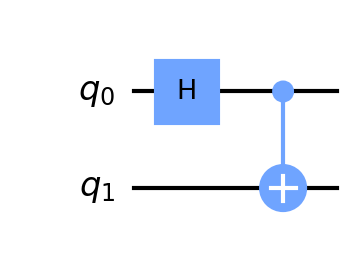
\includegraphics[scale=0.8]{./img/cx_gate.png}
\caption{\label{fig:orga04c113}CX Gate}
\end{figure}


\subsubsection{Dynamic Quantum Circuits}
\label{sec:org8b0e923}
\paragraph{Limitations of near-term quantum devices}
\label{sec:org9a4e2be}
This section discusses the limitations of near-term quantum
devices and shows that classical computing inside a quantum circuit is
for reaching the full potential of quantum computation.

\paragraph{Role of classical computing for quantum devices}
\label{sec:org31e2285}
I provide examples of how dynamic quantum circuits perform measurements
within a quantum circuit, how a classical computer collects these results,
processes them and then controls the subsequent quantum gates after the measurement.

\paragraph{Quantum Processing and Architecture}
\label{sec:org3408efc}

\subsection{Verification Tools for Quantum Circuits}
\label{sec:orga91866d}
Quantum computing has emerged as a promising technology for solving complex
problems that are beyond the capabilities of classical computers. However,
designing and verifying quantum circuits is a challenging task due to the
inherent complexity of quantum systems. 

Current approaches to address this challenge use Quantum Multiple-Valued
Decision Diagrams (QMDDs), Tensor Decision Diagrams or ZX-Calculus,
all of these approaches have been shown to be effective in
verifying the equivalence of quantum circuits, yet have different strengths 
and weaknesses. 

This literature survey aims
to provide an overview of the research on QMDDs, TDDs and ZX-Calculus for
equivalence checking and provides an describes how they are used for 
verifying the equivalence of quantum circuits.

\subsubsection{Quantum Multiple-Valued Decision Diagrams}
\label{sec:org5095817}
QMDDs are a type of decision diagram that can represent multiple values
simultaneously, making them suitable for representing quantum states \cite{Miller_QMDD_2006}. The
basic idea behind QMDDs is to represent a quantum state as a tree
structure, where each node represents a superposition of quantum states.
The edges of the tree represent the transitions between different
superpositions. By using QMDDs, it is possible to efficiently represent and
manipulate quantum states, which is essential for verifying the equivalence
of quantum circuits.

 Several studies have explored the use of QMDDs for verifying the equivalence of
 quantum circuits. 
 For example, in \cite{peham_equivalence_2022}, the authors proposed a method for
 verifying the equivalence of two quantum circuits by constructing their
 corresponding QMDDs and comparing them. 
 They showed that their method is
 efficient and scalable
\cite{Niemann_QMMD_2017} \cite{zulehner_advanced_2018}\cite{zulehner_efficiently_2019} , even for large
 quantum circuits. 
 In \cite{Burgholzer_random_2021}, the
 authors proposed a new technique for constructing QMDDs that reduces the
 number of nodes and edges required, thereby improving the efficiency of the
 verification process .

In conclusion, QMDDs have emerged as a powerful tool for verifying the
equivalence of quantum circuits. Several studies have explored the use of
QMDDs for this purpose, and have proposed new techniques for constructing,
manipulating and visualizing QMDDs \cite{Wille_tools_2022}. 

\subsubsection{TDD}
\label{sec:org90a6873}

\subsubsection{ZX-Calculus}
\label{sec:org9d653e5}

\section{Equivalence Checking of Quantum Circuits}
\label{sec:orgf9344d1}
\subsection{Equivalence Checking of traditional Quantum Circuits}
\label{sec:org23ea817}

\subsection{Equivalence Checking of dynamic Quantum Circuits}
\label{sec:org0631a3c}
\begin{itemize}
\item[{$\square$}] Discuss the specific challenges and methods for checking non-unitary quantum circuits.
\item[{$\square$}] Highlight the work of Burgholzer and Wille in ``Handling Non-Unitaries in Quantum Circuit Equivalence Checking.'' \cite{burgholzerHandlingNonunitariesQuantum2022}
\item[{$\square$}] Benchmark all Quantum Circuits from Extending the Design Space \cite{koleExtendingDesignSpace2023}

Dynamic quantum circuits contains non-unitary operations.
\end{itemize}

\subsubsection{Why verifying dynamic quantum circuits is different from verifying traditional quantum circuits}
\label{sec:org770c3c1}

\subsection{Equivalence Checking with the ZX-Calculus}
\label{sec:orgaded60e}
\begin{itemize}
\item[{$\square$}] Provide an in-depth explanation of the ZX-Calculus and its application in quantum circuit equivalence checking.
\begin{itemize}
\item What ZX-Calculus is
\item Simplification Rules
\item Reduction Rules
\item How to represent quantum circuits using ZX-Calculus
\item Equivalence Checking with a density matrix
\end{itemize}
\item[{$\square$}] Discuss the advantages and limitations of using ZX-Calculus for this purpose.
\item[{$\square$}] Present any findings from the analysis of ZX-Calculus tools.
\item[{$\square$}] Present limitations found in the ZX-Calculus Equivalence Checker
\end{itemize}

\subsection{Evaluation of existing equivalence checking tools}
\label{sec:orgb66acd2}
The verification of equivalence for dynamic circuits presents a unique and challenging problem.
Recent studies, highlighted in
\cite{burgholzerHandlingNonunitariesQuantum2022} and
\cite{hongEquivalenceCheckingDynamic2021} have explored various
approaches, such as the ZX-Calculus and Tensor Decision Diagrams. These
studies have revealed both strength and weaknesses in these methods,
suggesting that a combination of approaches may be the most effective
strategy. This is further discussed in chapter \hyperref[sec:org4f581f6]{Discussion and Future Work}.

Represent the implemted methods and evalutate how good they are
Experimental Resuls and evaluations
Finish 2 
implementation
Chapter 3

\subsubsection{Overview of the Study}
\label{sec:org57c9867}
This research aims to contribute empirical data to the field of dynamic
quantum circuit equivalence checking. The goal of this evaluation is to
obtain empirical data of the performance and capabilities of different
equivalence checking tools for quantum circuits. The collected results will
form the basis for a critical evaluation of existing verification tools.
This critique will not only shed light on the current state of equivalence
checking tools, but also provide valuable insight for researchers working
to enhance the accuracy and efficiency of tools for checking the
equivalence of dynamic quantum circuits. The study evaluates if these tools
can handle probabilistic circuits, the accuracy of the tool, its efficiency
and how it handles dynamic quantum circuits. This critic will guide
researches to improve the tools for checking the equivalence of dynamic
quantum circuits.

\subsubsection{Motivation}
\label{sec:orga2cccf9}
Improving equivalence checking tools for quantum circuits is beneficial for
correctness verification, hardware compilation, circuits optimization,
circuit design and helps researchers simulate, diagnose and fix errors in
quantum algorithms or hardware.

\subsubsection{Hypothesis}
\label{sec:orga09dc74}
The experiment data is composed of traditional quantum circuits with their
dynamic quantum counterparts of varying complexity. These pairs are either
equivalent, equivalen to a specific degree or not equivalent or
undecidable. Each quantum circuit pair will be evaluated by my own
implementation and publically available FOSS equivalence checking tools. I
expect to find, that the equivalence checking tools will have difficulties
with large quantum circuits and dynamic quantum circuits, which are
probabilistic. I this is because probabilistic quantum circuits
often are only equivalent to a specific degree including a different
global phase.

\subsubsection{Dataset}
\label{sec:org392ca1f}
The experimental dataset consists of traditional quantum circuits and their
dynamic counterparts, each with varying degrees of complexity. These pairs
fall into the categories of equivalence, equivalence to a specific degree,
non-equivalence or undecidable.

\subsubsection{Results}
\label{sec:org54cf13f}
The results of this evaluation provide us with a qualitative equivalence
assessment, a quantitative equivalence measurement and the time required
for verifying the equivalence of the quantum circuit pair. These findings
are anticipated to provide valuable data for critical evaluating existing
equivalence checkers and, potentially, for proposing new approaches for
checking the equivalence of quantum circuits. By analysing strengths and
weaknesses of these tools, this thesis aims to contribute to the ongoing
development and improvement of quantum circuit equivalence checking
methodologies.


\subsubsection{Method}
\label{sec:org288613f}
This empirical study involves the integration of different quantum circuit
equivalence checking tools.
I choose to base my evaluation on the quantum circuits, which have been
generated by an algorithm, which transforms traditional quantum circuits into
dynamic quantum circuits \cite{koleExtendingDesignSpace2023}. The goal of
this algorithm is to reduce the quantum cost of implementing these circuits.
The algorithms presented transform traditional quantum circuits with \(n\)
qubits into dynamic circuits with \(2\) circuits in the best case. Thus, the
quantum cost is reduced by tansforming traditional quantum circuits into
dynamic quantum circuits.


\subsubsection{Setup}
\label{sec:orgbdae092}

The benchmarks are integrated into `QuantumCircuitEquivalence.jl` a Julia
package I have developed during the research phase of my thesis. For
automatic benchmarking of the different equivalence checking tools, it uses
the `PyCall` library to integrate serveral equivalence checkers which provide a
python API. This library allows `QuantumCircuitEquivalence.jl` to share
memory with any python object or function allowing me to integrate
\emph{mqt-qcec} and qiskit into \emph{QuantumCircuitEquivalence.jl}. Calling the
quantum circuit equivalence checkers directly from
`QuantumCircuitEquivalence.jl` allows me to automatically perform the
 benchmark without any manual steps. If at any step I want to add more
 circuits to benchmark, I can just add the QASM files to the benchmark
 folder, and they will be included in the benchmark in any later evaluation.


Each equivalence checking tool will be tasked to verify the equivalence of a dynamic quantum
circuit and a traditional quantum circuit which both are provided in the \emph{OpenQASM} file format.


I have chosen to evaluate  the different equivalence checkers of \emph{mqt-qcec}
 (decision digrams, alternative, construction, simulation, ZX-Calculus),
 MQT's approach for dynamic quantum circuit chooses to transform non-unitary
 quantum circuits (dynamic) into unitary quantum circuits and then use
 existing methods for checking the equivalence of unitary quantum circuits.
 Qiskit provides different equivalence checkers and is widely used by
 quantum computers researchers. I have included their equivalence checking
 methods since I am interested in how it handles non-unitary circuits and
 large quantum circuits with more than 30 qubits.


The selection of the
equivalence checking tools will be based on criteria such as their
popularity in the field, availability of source code and their
compatibility with circuits under examination.


\subsubsection{Data}
\label{sec:org9b10e65}
\begin{verbatim}
using QuantumCircuitEquivalence
using QuantumCircuitEquivalence.Operator

benchmark_equivalence_checking()
\end{verbatim}

\subsubsection{Discussion of Results}
\label{sec:orga2e94b6}
\section{Discussion and Future Work}
\label{sec:org4f581f6}

\section{Conclusion}
\label{sec:orge6e3725}
\begin{itemize}
\item[{$\square$}] Summarize the key points of the thesis.
\item[{$\square$}] Reiterate the importance of this research in the context of quantum computing.
\end{itemize}

\section{Appendix}
\label{sec:org46d2c69}

\bibliographystyle{ieeetr}
\bibliography{refs.bib}




\printglossaries
\listoffigures
\listoftables


\subsection{Table of Acronyms (Acronyms)}
\label{sec:orga59bb5b}

\subsection{Table of Glossaries (Glossary)}
\label{sec:org8bc0727}

\newpage


\subsection{Mathematical Foundations}
\label{sec:org9d349e2}
All the following mathematical definitions have been adapted mathematical foundations chapter of \cite{hayashi_introduction_2015}

\subsubsection{Dirac Notation}
\label{sec:orgafd391e}
The Dirac or bra-ket notation is a notation for linear algebra and linear operators on complex vector spaces.
Its design goal is to ease frequent calculation which occur in quantum mechanics.

Kets are vectors in the Hermitian Vector Space.

These are our Basis States in the Z-Basis:
\begin{itemize}
\item Zero \(\ket{0} = \myvec{0 \\ 1}\)
\item One \(\ket{1}i = \myvec{1 \\ 0}\)
\end{itemize}

with the following properties:
\begin{itemize}
\item \(\braket{u}{v}=\braket{v}{u}^\star\)
\item \(\braket{v}{v}\geq 0\) \(\forall\) \(\ket{v}\)
\item \(\braket{v}{v}= 0\) if and only if \(\ket{v}=0\)
\end{itemize}

\subsubsection{Daggers}
\label{sec:org615cf3f}
Any Matrix \(M\) can be transposed, then complex conjugated as \(M^\dagger\).
This operation is referred to as a hermitian conjugation in quantum
mechanics or as the conjugate transpose in linear algebra.
A dagger is a bijective map between the \(\mathbb{H}\) and \(\mathcal{H}^*\) space
given by \(\ket{v} \leftrightarrow \bra{v}\)
$$\bra{v} = (\ket{v})^\dagger$$
$$\ket{v} = (\bra{v})^\dagger$$

When applied twice the dagger operation is the identity map \(I\).


\subsubsection{Geometry}
\label{sec:org7e4dab3}

\paragraph{Norm or Length}
\label{sec:orgb833de2}
The length or norm of \(\ket{v}\) is \(||v|| = \sqrt{\braket{v}{v}}\).
Two Kets \(\ket{u}\) and \(\ket{v}\) are orthogonal if \(\braket{v}{u} = 0\).


\paragraph{Orthogonal basis}
\label{sec:orge9a3dd7}
Any vector can be expressed as a linear combination of the basis vectors:
$$ \ket{v} = \sum_i{v_i \ket{e_i}} \text{ where } v_i = \braket{v}{e_i}$$.

The bras form \(\bra{e_i}\) form a dual basis:
$$\bra{v} =  \sum_i{v_i^* \bra{e_i}} \text{ where } v_i^* = \braket{e_i}{v}$$.

\paragraph{Minimal Spanning Set}
\label{sec:orgf9b81f4}

\subsubsection{Eigenvalues and eigenvectors}
\label{sec:orgf211f2a}
Given any operator \(A\), an eigenvector is defined as a non-zero vector \(\ket{v}\), with
the following property:
$$A\ket{v} = \lambda \ket{v} | \lambda \in \mathbb{C}$$
Where \(\lambda\) is refered to as the corresponding \textbf{eigenvalue}.

\subsubsection{Outer Product}
\label{sec:org741d54a}
The outer product \(\ketbra{u}{v}\) is a linear map on the Hilbert space \(\mathbb{H}\)

Any Operator on the Hilbert Space \(\mathbb{H}\) can be rewritten as the sum of outer products.

\subsubsection{The trace}
\label{sec:org7d7d55b}
A \textbf{trace} operation turn an outer product into an inner product.

$$tr: \ketbra{b}{a} \rightarrow \braket{a}{b}$$

The trace of a square matrix \(A\), is defined as the sum of its diagonal elements:
$$tr A = \sum{\bra{e_k}A\ket{e_k}} = \sum_k{A_{kk}}$$.


\subsubsection{Tensor Product}
\label{sec:org358aa39}
\paragraph{Vector Spaces}
\label{sec:org1381136}
The tensor product is a way of putting vector spaces together to form larger
vector spaces. It is fundamental building operation of quantum system. If
\(V\) describes one quantum system and \(V^\prime\) describes another, then
their tensor product describes both quantum systems as one. It is
important to remember, that a vector can be written as the tensor of two
vectors (separable) and some vectors cannot be written as the tensor of
two vectors, due to \textbf{entanglement}.

To obtain a tensor product of two vectors multiply each element of the
vectors together and then stack them.
\paragraph{Matrices}
\label{sec:org8c8405e}
The Kronecker Product is a special version of the tensor product. It is used for obtaining
the tensor product of two matrices \(A\) and \(B\). Definition of the Kronecker Product:
$$
     \mathbf{A}\otimes\mathbf{B} = \begin{bmatrix}
       a_{11} \mathbf{B} & \cdots & a_{1n}\mathbf{B} \\
                  \vdots & \ddots &           \vdots \\
       a_{m1} \mathbf{B} & \cdots & a_{mn} \mathbf{B}
     \end{bmatrix}
     $$


\subsubsection{Hilbert Space \(\mathbb{H}\)}
\label{sec:org36afc5a}
Hilbert's space is a linear vector space of complex number, where a
\textbf{complex inner product} is defined \(\bra{\psi_i}\ket{\psi_j} =
    \delta_{ij}\), and the transformation is linear.


\textbf{Two conditions} of the Hilbert Space
\begin{description}
\item[{Normalized}] Sum of eigenvector always \(\vec{i} \cdot \vec{i} = \vec{j} \cdot \vec{j} = \vec{k} \cdot \vec{k}= 1\)
\item[{Orthgogonal}] Sum of e i != j always \(\vec{i} \cdot \vec{j} = \vec{j} \cdot \vec{k} = \vec{k} \cdot \vec{i}= 0\)
\end{description}



\paragraph{Operators}
\label{sec:org60ff678}
A \textbf{linear map} is a function \(A: \mathbb{H} \rightarrow K\) between the vector space \(\mathcal{H}\) and \(\mathcal{K}\),
which respects linear combinations:
$$A(c_1 \ket{v_1} + c_2\ket{v_2}) = c_1 A \ket{v_1} + c_2 A \ket{v_2}$$
where \(\ket{v_1}, \ket{v_2}\) are vectors and \(c_1, c_2\) are complex numbers.

To obtain the product \(BA\) of the operators \(A\) and \(B\), first \(A\) is applied to
a ket \(\ket{v}\) and then \(B\)  is applied to the result from the application of \(A\):

$$(BA)\ket{v} = B(A\ket{v})$$

Any evolution of a quantum system is represented by a unitary operator, which preserves
the inner product. Given a unitary operator \(U\)  and two kets \(\ket{a}\) and \(\ket{b}\),


\paragraph{Inner Product}
\label{sec:org5cb23fa}
The inner product is a scalar product. It is the \textbf{probability amplitude} of finding state \(\psi_f\) after measuring on the state \(\phi_i\)

\paragraph{Outer Product}
\label{sec:org6103e5c}
There is a useful way of representing linear operators that makes use of
the inner product, known as the outer product representation.Suppose
\(\ket{v}\) is a vector in an inner product space \(V\), and \(\ket{w}\) is a
vector in an inner product space \(W\)

\textbf{What is the outer product:}
\begin{itemize}
\item The outer product is a projection operator.
\item The trace of the outer product of \(\psi_i, \psi_j\) equals the inner product of \(\psi_i, \psi_j\)
\item For any orthonormal basis \(\ket{i}\), we can show that:
$$\sum_{i} \ket{i}\bra{i} = I$$
\end{itemize}

\subsubsection{Quantum Projection Operation}
\label{sec:org13885d2}
 Quantum Projection Operator can:
\textbf{A projection operator project any vector \(\vec{v}\) onto the subspace of another vector \(\vec{o}\)}

\paragraph{Measurement Basis}
\label{sec:orgc3182bf}
A \textbf{minimal spanning set} is referred to as a basis.

\paragraph{Properties of a Projection Operator}
\label{sec:org8fba414}
\begin{description}
\item[{Symmetric}] \(A = A^T \mid A \in \mathbb{R}^{n \times n}\)
\item[{Hermitian}] \(\vec{P_u^\dagger} = \vec{P_u} \mid P \in \mathbb{R}^{n \times n}\)
\item[{Completness Rule}] \(\vec{P_u^2} = \braket{u}{u}\braket{u}{u} = \braket{u}{u} = \vec{P_u}\)
\item[{System}] \(\sum\vec{p} = I\)
\end{description}

\paragraph{Properties of a Unitary Matrix}
\label{sec:orgac316c3}
All quantum gate operations can be represented as unitary matrices. For a
matrix to be unitary, this property needs to hold:
$$U \times U^\dagger = U^\dagger \times U = I_n \mid U \in \mathbb{R}^{n \times n}$$.

\paragraph{Important Rules for Unitary Matrices}
\label{sec:orgaeada06}
\begin{itemize}
\item If \(U_1\) and \(U_2\) are unitary matrices, so is their matrix product \(U_1 \cdot U_2\)
\item Unitary matrices preserve inner products. Thus if \(U\) is unitary, then for all \(V, V^\prime \in \mathbb{C}^n\) we have:
$$\braket{UV}{UV^\prime} = \braket{U}{V^\prime}$$
\end{itemize}

\paragraph{Schrödinger Equation}
\label{sec:orgea3b168}
\begin{equation}
i\hbar\frac{\partial}{\partial t} \Psi(x,t) = \left [ - \frac{\hbar^2}{2m}\frac{\partial^2}{\partial x^2} + V(x,t)\right ] \Psi(x,t)
\end{equation}

\paragraph{Common Gates}
\label{sec:org787618d}
\begin{figure}[htbp]
\centering
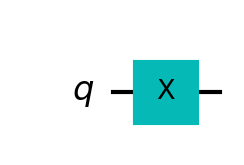
\includegraphics[scale=0.8]{./img/x_gate.png}
\caption{X Gate}
\end{figure}

\begin{equation}
\begin{bmatrix}
  \\[0pt]
\end{bmatrix}
\end{equation}

\subsubsection{Multi Qubit Gates}
\label{sec:orgba18d6c}

\subsubsection{Reversible Computing}
\label{sec:org388d21e}
Reversible computing means given the operation and output value, you can
find the input value For \(A x= b\), given \(A\) and \(b\), you can find \(x\).
Their function is bijective.
Operations which permute are reversible; operations which erase and overwrite are not.
For Example identity and negation are reversible, constants are not reversible.
\end{document}